\section*{Abstract}
This report studies the Delaunay's triangulation, more explicitly the Watson's algorithm depicted in \cite{de2000computational}, and comes to explain and illustrate our implantation written in the code : 
\begin{table}[h!]
\centering
\begin{tabular}{c|cc}
C code & name of the file & description \\
\hline
Launch  & \texttt{main.c} & launch the code \\
Main  & \texttt{watson.c}, \texttt{watson.h} & implementation of the Watson's algorithm \\
Robust library & \texttt{robustFunctions.c} & see section "robustness" \\
GUI & \texttt{glfem.c}, \texttt{glfem.h}, \texttt{graphic.c} & implementation of the graphic interface \\
\hline
\hline
Matlab code & & \\
\hline 
 Random& \texttt{generatePointRandom.m} & function to write random points into binary files\\
 Limit  & \texttt{generatePointLimite.m} & function to write worst case scenario points into binary files \\
 Results & \texttt{time.m}				& script to get the results of the report\\
 \hline
\hline
User intervention & & \\
\hline
Make 	& \texttt{make} & Adapt the Makefile for your computer \\
Launch  & \texttt{./myDelaunay a b c d} & Launch the Triangulation with the options \\
Remove  & \texttt{rm data/*} 			& Remove the files gerenatered for evolution
\end{tabular}
\end{table} 

The parameters required with \texttt{./myDelaunay} are the following
\begin{enumerate}[label=\textbf{\alph*}]
\item = 1 if the user want to deal with worst case scenario, = 0 otherwise;
\item = 1 if the user want to use the most robust implementation, = 0 otherwise ;
\item = 2 if the user want the final graph of the triangulation, \\ = 1 if he wants the evolution point by point, \\= 0 otherwise (no graph)  ;
\item = 1 if the user want to randomise the list of points received, = 0 otherwise.
\end{enumerate}

We first present the the whole algorithm and the data structures related to it. Then we present the architecture of our codes. We go ahead with a deep insight in the robustness question. Finally we present the performance results of our code. 


\newpage
\section{Delaunay's triangulation : Watson's algorithm}
Watson's algorithm \cite{de2000computational} is a randomized incremental algorithm : we first build a "big triangle" containing all the points, then we add the points one by one maintaining the Delaunay's properties at each step. The input is an list of points containing the $x$ and $y$ coordinates of each one. The output is a list of $n$ triangles (i.e. $n$ lines and $3$ column containing indices of the nodes).

\subsection*{Data's structures}
We have seven data's structures as depicted in figure \ref{fig:dataStruct} and implemented in \texttt{watson.h}.

\begin{figure}[h!]
\centering
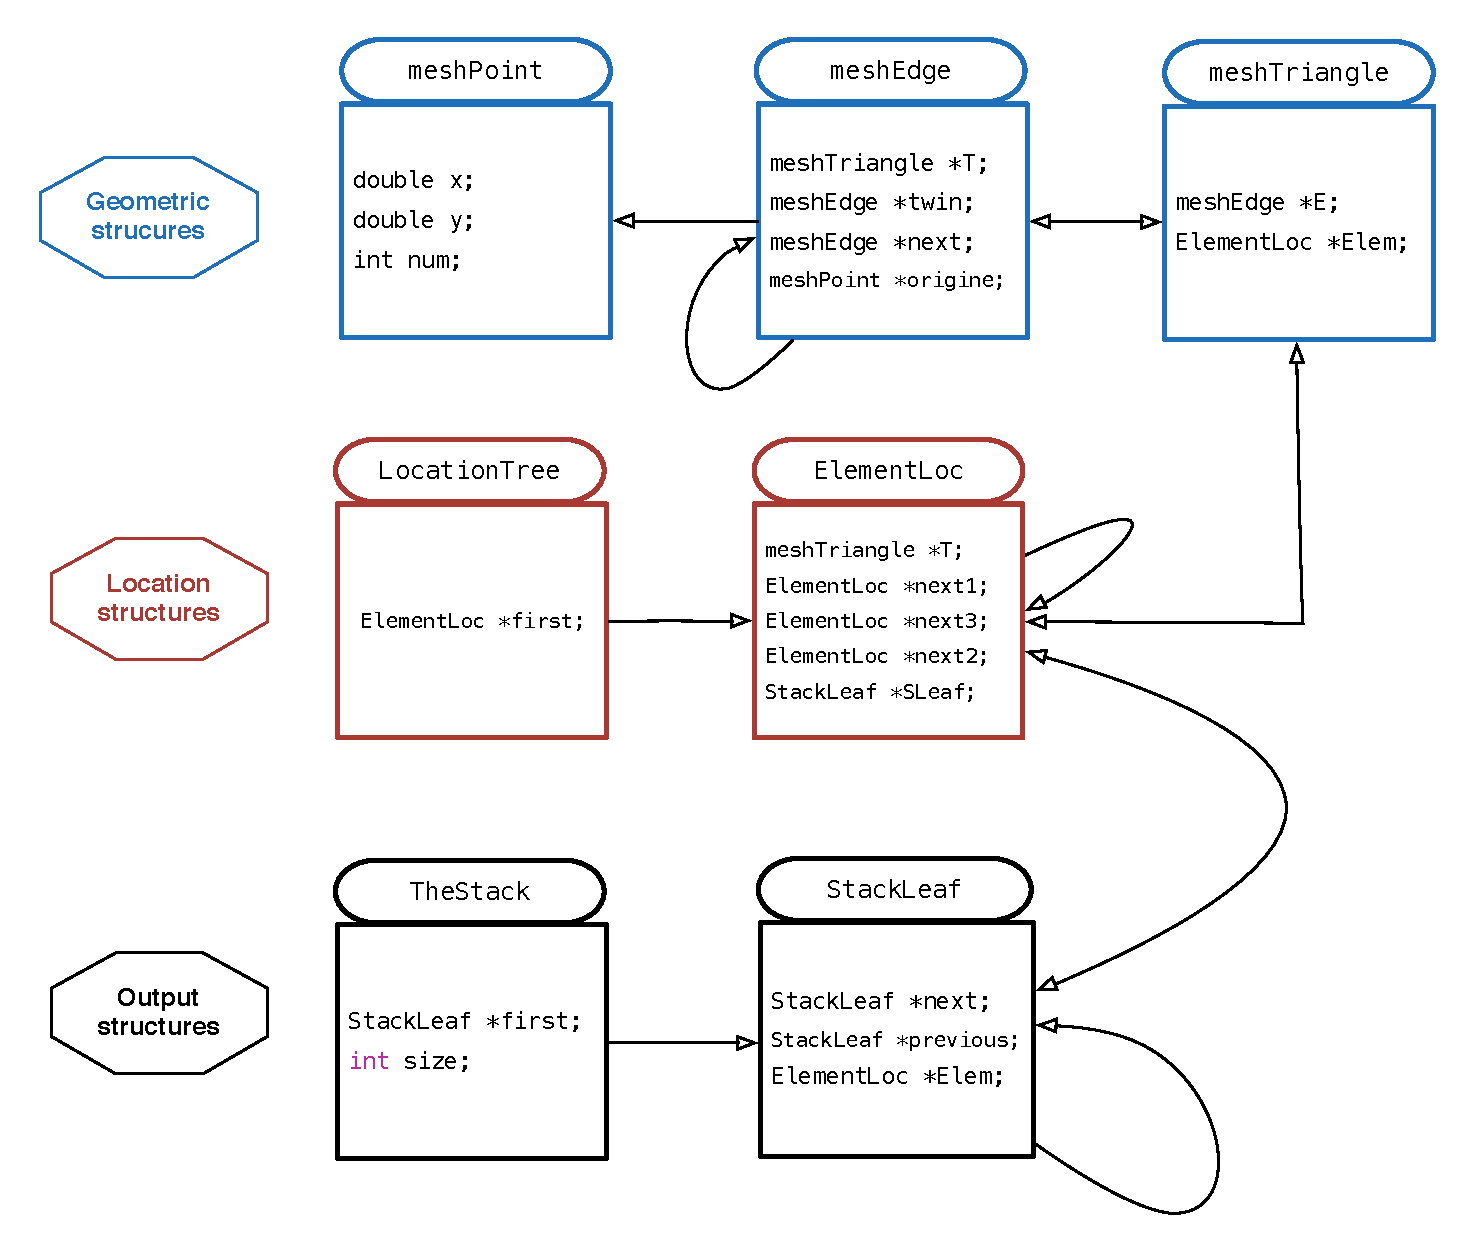
\includegraphics[width=0.8\textwidth]{images/dataStruct.eps}
\caption{Data structures of our code.}
\label{fig:dataStruct}
\end{figure}

We divided them into three categories: 
\begin{itemize}
\item the geometric structures contain all the informations about the mesh itself : the nodes, the triangles and the points. Note that each triangle has its own edges ordered counter-clockwise; therefore, a triangle only need to know one of its edge, from which it can reach the other edges, points... The structure of the edges is the one which makes the links between points and triangle and also between neighbour triangles (as \texttt{meshEdge} contain a pointer toward its \texttt{twin} which contain a pointer toward its \texttt{meshTriangle});
\item the location structure, more precisely the location tree, denoted later as $\mathcal{T}$. This structure works as follow : its first element is the "big triangle"; then when we add a point $p_r$, we create new triangles which are the \texttt{next} elements of the "parent" element in the tree. So each \texttt{ElementLoc} has three pointer toward the 3 next \texttt{ElementLoc}, a pointer toward the triangle it represents and a pointer toward its potential element in the stack;
\item  the stack structures, denoted later as $\mathcal{S}$, which contains at each step, the leaves of the location tree $\mathcal{T}$. This structure is useful because it allows us to easily return the leaves of the the tree (so the final mesh, the output of the algorithm) at the end of the algorithm. It is also useful to plot the evolution of the mesh (cf. the GUI). 
\end{itemize}
 

\subsection*{Watson's algorithm}
Our algorithm can be written as follow :  
\begin{algorithm}[h!]
\caption{Watson-DelaunayTriangulation($\mathcal{P}$)}\label{Delaunay}
\begin{algorithmic}[1]
\State \textit{Input} A set of $n$ points $\mathcal{P}$
\State \textit{Output} An array of Delaunay's triangles
\State Initialise the "big triangle" by choosing three extreme points 
\State Initialise the data's structures (the location tree $\mathcal{T}$ and the stack $\mathcal{S}$)
\State perform a random permutation on $\mathcal{P}$
\For {$r \gets 1$ \textbf{to} $n$}
\State Find triangle $p_ip_jp_k \in \mathcal{T}$ containing $p_r$
\If {$p_r$ lies in the interior of triangle $p_ip_jp_k$} 
\State Add edges from $p_r$ to $p_i$, $p_j$ and $p_k$ and create three new triangles. Add them to the structure $\mathcal{T}$ and actualise $\mathcal{S}$.
\State Legalize edge ($p_r$, $\overline{p_ip_j}$,triangle $p_ip_jp_r$,$\mathcal{S}$)
\State Legalize edge ($p_r$, $\overline{p_jp_k}$,triangle $p_rp_jp_k$,$\mathcal{S}$)
\State Legalize edge ($p_r$, $\overline{p_kp_i}$,triangle $p_ip_rp_k$,$\mathcal{S}$)
\Else ($p_r$ lies on an edge of triangle $p_ip_jp_k$, say $p_ip_j$)
\State Add edges from $p_r$ to $p_k$ and to $p_l$ (the opposite node in the adjacent triangle $p_ip_jp_l$) and create four new triangles. Add them to $\mathcal{T}$ and actualise $\mathcal{S}$.
\State Legalize edge ($p_r$, $\overline{p_ip_l}$,triangle $p_ip_rp_l$,$\mathcal{S}$)
\State Legalize edge ($p_r$, $\overline{p_lp_j}$,triangle $p_rp_jp_l$,$\mathcal{S}$)
\State Legalize edge ($p_r$, $\overline{p_jp_k}$,triangle $p_rp_jp_k$,$\mathcal{S}$)
\State Legalize edge ($p_r$, $\overline{p_kp_i}$,triangle $p_ip_rp_k$,$\mathcal{S}$)
\EndIf
\EndFor
\Return $\mathcal{S}$
\end{algorithmic}
\end{algorithm}

where the step "legalize edge" corresponds to : 
\begin{algorithm}[h!]
\caption{Legalize Edge($p_r$, $\overline{p_ip_j}$, triangle $p_ip_jp_r$,$\mathcal{S}$)} \label{legalizeEdge}
\begin{algorithmic}[1]
\State Let $p_ip_jp_k$ be the adjacent triangle to $p_ip_jp_r$. Test if $p_k$ lies inside the oriented circle define by $p_ip_jp_r$. If it is the case, $\overline{p_ip_j}$ is illegal 
\If {$\overline{p_ip_j}$ is illegal } 
\State create a new edge $\overline{p_rp_k}$ and create two new triangles associated. Add them to the structure $\mathcal{T}$ and actualise $\mathcal{S}$.
\State Legalize edge ($p_r$, $\overline{p_ip_k}$,triangle $p_rp_ip_k$,$\mathcal{S}$)
\State Legalize edge ($p_r$, $\overline{p_kp_j}$,triangle $p_rp_jp_k$,$\mathcal{S}$)
\EndIf
\end{algorithmic}
\end{algorithm}

More explicitly for the initialisation of the "big triangle": 
\begin{verbatim}
thePoint[0] = meshPointCreate(minX - 10*(maxX-minX),minY-10*(maxY-minY),0);
thePoint[1] = meshPointCreate(maxX + 10*(maxX-minX),minY-10*(maxY-minY),1);
thePoint[2] = meshPointCreate((maxX+minX)/2,maxY+10*(maxY-minY),2);
\end{verbatim}

Our implementation is in the files \texttt{watson.c}.
This algorithm is expected to run in $O(n \log n)$ time in most cases and $O(n^2)$ in "worst" cases (see \cite{de2000computational}). We will go back on this later.

\newpage